\providecommand{\pgfsyspdfmark}[3]{}
\providecommand{\savepicturepage}[3]{}

\documentclass[11pt,letterpaper]{article}
\usepackage[lmargin=1in,rmargin=1in,tmargin=1in,bmargin=1in]{geometry}

% -------------------
% Packages
% -------------------
\usepackage{
	amsmath,			% Math Environments
	amssymb,			% Extended Symbols
	enumerate,		    % Enumerate Environments
	graphicx,			% Include Images
	lastpage,			% Reference Lastpage
	multicol,			% Use Multi-columns
	multirow,			% Use Multi-rows
	gensymb
}


% -------------------
% Font
% -------------------
\usepackage[T1]{fontenc}
\usepackage{charter}
\usepackage{xcolor}

% -------------------
% Commands
% -------------------

\newcommand{\prob}{\noindent\textbf{Problem. }}
\newcounter{problem}
\newcommand{\problem}{
	\stepcounter{problem}%
	\noindent \textbf{Problem \theproblem. }%
}
\newcommand{\answer}{\noindent \textbf{Answer. }}
\newcommand{\pspace}{\par\vspace{\baselineskip}}
\newcommand{\ds}{\displaystyle}


% -------------------
% Header & Footer
% -------------------
\usepackage{fancyhdr}

\fancypagestyle{pages}{
	%Headers
	\fancyhead[L]{}
	\fancyhead[C]{}
	\fancyhead[R]{}
\renewcommand{\headrulewidth}{0pt}
	%Footers
	\fancyfoot[L]{}
	\fancyfoot[C]{}
	\fancyfoot[R]{}
\renewcommand{\footrulewidth}{0.0pt}
}
\headheight=0pt
\footskip=14pt

\pagestyle{pages}


% -------------------
% Content
% -------------------
\begin{document}
\noindent\textbf{\large Calculus I (AM\_\_1050AH / MSF\_10110) \\ 2022 Fall \\ Application of Derivatives (5.2-5.3)}

\bigskip

\noindent Note that in problems for related rates, you should clearly indicate the unit of your answer. 

\bigskip

\problem Let $f(x) = x^2 - 10x + 9$,
\begin{enumerate}[(a)]
    \item Find the roots of $f(x)$ using factorization.
    \item Find the roots of $f(x)$ using Newton's method, with initial guess set as $10$ and tolerance set at $10^{-5}$.  How many iterations was needed to reach tolerance?
    \item Find the roots of $f(x)$ using Newton's method, with initial guess set as $6$ and tolerance set at $10^{-5}$.  How many iterations was needed to reach tolerance?
    \item Compare the number of iteration in (b) and (c) and provide an explanation for their difference.
\end{enumerate}\vspace{6mm}


\noindent\begin{minipage}{0.7\textwidth}
    \problem A kid is holding a balloon with a string of length $150$ centimeters, and the balloon is now of height $90$ centimeters, shown in the graph on the right. Suppose the string is always taut, and the balloon is floating upwards with its height increasing by $15$ cm per second.  At what rate is the angle $\theta$ increasing?
\end{minipage}
\begin{minipage}{0.3\textwidth}
    \begin{center}
        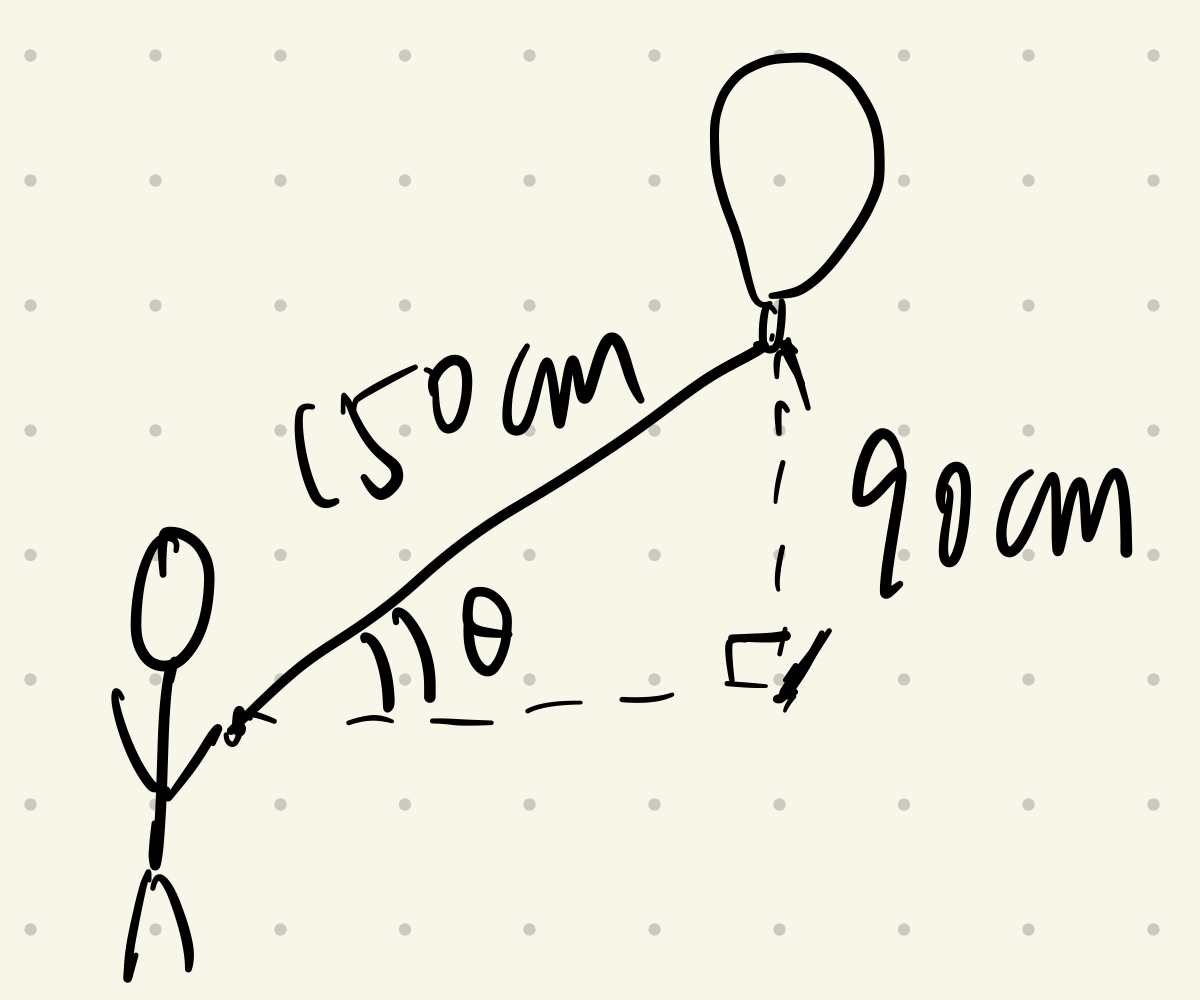
\includegraphics[width = 0.8\textwidth]{../graph/A11.png}
    \end{center}
\end{minipage}
\vspace{6mm}

\problem A sake bottle shaped like a cone is of radius $7$ cm at the bottom with height $10.5$ cm,
\begin{enumerate}[(a)]
    \item It is known that the volume of a cone with radius $r$ at the bottom and height $h$ is $\frac{1}{3}\pi r^2 h$.  Calculate the amount of sake in the bottle when the fluid level is $X$ cm from the bottom.
    \item Suppose we are pouring sake into the bottle at a constant speed of $30 \pi \approx 94.25$ cc/seconds.  If the current fluid level is just $3$ cm from the bottom, how fast is the fluid level rising now?
    \item From (b), if the current fluid level is $9$ cm from the bottom instead, how fast is the fluid level rising now?
\end{enumerate}\vspace{6mm}

\problem A good's \textit{price elascity of demand} measures the sensitivity of its quantity demanded relative to its price.  Let $P$ be the unit price of the good and $Q$ be the demanded quantity, where $P$ and $Q$ are related by the demand curve.  The point price elasticity of demand $E$ is defined as 
\[E = -\frac{dQ}{dP}\frac{P}{Q}\]
Suppose a good has current unit price of $\$500$ and its monthly demand is $1000$ units per month. If its point price elasticity is fixed at $1.5$ and its price is raised at a speed of $\$5$ per unit per month, at what rate is its quantity demanded changing?
\vspace{6mm}

% \problem Use the hinted linear approximations to approximate the following quantities:
% \begin{enumerate}[(a)]
%     \item $\tan 46 \degree$, approximating $\tan x$ at $x = 45 \degree$. (Note: You'll have to operate in radians) 
%     \item $\ln(1.01)$, approximating $\ln (1+x)$ at $x = 0$.
%     \item $\tan^{-1}0.99$, approximating $\tan^{-1} x$ at $x = 1$.
%     \item $\sqrt[4]{80}$, approximating $3\sqrt[4]{1+x}$ at $x = 0$.
%     \item $\frac{1}{0.99^3}$, approximating $\frac{1}{(1+x)^3}$ at $x = 0$.
% \end{enumerate}\vspace{6mm}

% \problem Find the following limits. You \textit{may} use the L'Hôpital's rule \textit{if applicable}.
% \begin{enumerate}[(a)]
%     \item $\lim\limits_{x \to 1} \frac{x^3+x^2+x-3}{x^3+2x^2+x-3}$
%     \item $\lim\limits_{x \to 0} \frac{e^{(3x^2+2x)}-1}{\sin(2x^2+3x)}$
%     \item $\lim\limits_{x \to 0} \frac{\sin (x^2)}{x \tan x}$
%     \item $\lim\limits_{x \to 0} x^2 \ln (x^2)$ \quad (Hint: Transform it into $\frac{\infty}{\infty}$ form)
%     \item $\lim\limits_{x \to 0} \frac{e^{-\frac{1}{x^2}}}{x^2}$ \quad (Hint: $\frac{0}{0}$ form can also be transformed into $\frac{\infty}{\infty}$ form)
% \end{enumerate}\vspace{4mm}

% \problem Determine if the following statements are true or false and explain. (You can just provide a counterexample if you determine them as false)
% \begin{enumerate}[(a)]
%     \item If $f'(x) = g'(x)$ (for all $x\in \mathbb{R}$), then $f(x) = g(x)$
%     \item If $f(1) = 0$, then $f'(1) = 0$
%     \item If $f'(x) = 0$ (for all $x\in \mathbb{R}$), then $f(x) = 0$
% \end{enumerate}\vspace{6mm}

% \problem Let $f(x) = \sqrt[4]{x} - \sqrt{x}$,
% \begin{enumerate}[(a)]
%     \item Find the tangent line of $f(x)$ at the point where $x=16$.
%     \item At which point(s) on $f(x)$ is its tangent line horizontal?
%     \item Is $f(x)$ differentiable at $x = 0$? Why?
% \end{enumerate}\vspace{6mm}

% \problem A ball is expanding with its radius $r$ as a function of time $t$: $r(t) = \sqrt{t} + 2, t \ge 0$
% \begin{enumerate}[(a)]
%     \item Find the rate its radius is growing at $t = 1$
%     \item Find the rate its surface area is growing at $t = 1$
%     \item Find the rate its volume is growing at $t = 1$
% \end{enumerate}\vspace{6mm}

\end{document}